\documentclass[12pt,letterpaper]{article}

%%%%%%%%%%%%%%%%%%%%%%%%%%%%%%%%%%%%%%%%%%%%%%%%%%%%%%%%%%%%%%%%%%%%%%%%%
\pagestyle{plain}                                                      %%
%%%%%%%%%% EXACT 1in MARGINS %%%%%%%                                   %%
\setlength{\textwidth}{6.5in}     %%                                   %%
\setlength{\oddsidemargin}{0in}   %% (It is recommended that you       %%
\setlength{\evensidemargin}{0in}  %%  not change these parameters,     %%
\setlength{\textheight}{8.5in}    %%  at the risk of having your       %%
\setlength{\topmargin}{0in}       %%  proposal dismissed on the basis  %%
\setlength{\headheight}{0in}      %%  of incorrect formatting!!!)      %%
\setlength{\headsep}{0in}         %%                                   %%
\setlength{\footskip}{.5in}       %%                                   %%
%%%%%%%%%%%%%%%%%%%%%%%%%%%%%%%%%%%%                                   %%
\newcommand{\required}[1]{\section*{\hfil #1\hfil}}                    %%
\renewcommand{\refname}{\centerline{References Cited}}                 %%
\bibliographystyle{plain}                                              %%
%%%%%%%%%%%%%%%%%%%%%%%%%%%%%%%%%%%%%%%%%%%%%%%%%%%%%%%%%%%%%%%%%%%%%%%%%

%PUT YOUR MACROS HERE

\usepackage{graphicx}
\usepackage{subfigure}
\usepackage{amsmath}
\usepackage{amssymb}
\usepackage{times}
\usepackage{enumitem}
\usepackage{mathrsfs}
\usepackage[sort, compress]{natbib}
\usepackage{float}
\usepackage[ruled,vlined]{algorithm2e}
\usepackage{fixltx2e,dblfloatfix}
\usepackage{url}


\DeclareMathOperator*{\argmin}{argmin}
\DeclareMathOperator*{\argmax}{argmax}
\DeclareMathOperator*{\N}{\mathcal{N}}
\newcommand{\mbf}[1]{\mathbf{#1}} %note: I think using \mb killed the UF thesis template, changed to \mbf
\def\m{\textrm{m}}
\def\x{\mathbf{x}}
\def\t{\mathbf{t}}
\def\K{\mathbf{K}}
\def\y{\mathbf{y}}
\def\e{\mathbf{e}}
\def\p{\mathbf{p}}
\def\s{\mathbf{s}}
\def\b{\mathbf{b}}
\def\w{\mathbf{w}}
\def\n{\mathbf{n}}
\def\a{\mathbf{a}}
\def\u{\mathbf{u}}
\def\z{\mathbf{z}}
\def\B{\mathbf{B}}
\def\C{\mathbf{C}}
\def\E{\mathbf{E}}
\let\sec\S
\def\S{\mathbf{S}}
\def\I{\mathbf{I}}
\def\P{\mathbf{P}}
\def\X{\mathbf{X}}
\def\A{\mathbf{A}}
\def\C{\mathbf{C}}
\def\M{\mathbf{M}}
\def\U{\mathbf{U}}
\def\Y{\mathbf{Y}}
\def\Z{\mathbf{Z}}
\def\balpha{\boldsymbol\alpha}
\def\bmu{{\boldsymbol\mu}}
\def\btheta{{\boldsymbol\theta}}
\def\bSigma{\mathbf{\Sigma}}
\def\hbmu{\hat{\bmu}}
\def\hbSigma{\hat{\bSigma}}
\def\bTheta{\boldsymbol\Theta}
\def\bLambda{\boldsymbol\Lambda}
\def\del{\partial}
\newcommand{\bb}[1]{\textbf{#1}}

\usepackage[uppercase]{titlesec}
\titleformat{\section}{\bfseries \scshape \large }{\thesection}{1em}{}
\titleformat{\subsection}{\bfseries \scshape}{\thesubsection}{1em}{}
\titleformat{\subsubsection}{\bfseries \scshape}{\thesubsubsection}{1em}{}
\titleformat{\paragraph}{\bfseries}{}{1em}{}
\titlespacing*{\section}{0pt}{5pt}{0pt}
\titlespacing*{\subsection}{0pt}{5pt}{0pt}
\titlespacing*{\subsubsection}{0pt}{5pt}{0pt}
\titlespacing*{\paragraph}{0pt}{5pt}{0pt}



\title{Kernels \& the Dual Form }

\begin{document}
\maketitle

\section{Introduction to Kernels}
\begin{itemize}

\item One main idea behind using kernels is to go into a higher dimensional space where it might be easier to segment or analyze the structure of the data.  

\item \text{Inner product:} Let $H$ be vector space over $\mathbb{R}$.  A function $<\cdot, \cdot>_H : H\times H \rightarrow \mathbb{R}$ is an inner product in $H$ if
\begin{enumerate}
\item $\left<a_1f_1 + a_2f_2, g\right>_H = a_1\left<f_1, g\right>_H + a_2\left<f_2, g\right>_H$

\item $\left<f,g\right>_H = \left<g,f\right>_H$

\item $\left<f,f\right>_H \ge 0 \text{ and } \left<f,f\right>_H = 0 \iff f = 0$
\end{enumerate}

\item Essentially, a Hilbert space is a (complete metric) space where an inner product is defined.  

\item \textbf{Kernel:} Let $X$ be a non-empty set.  A function $k: X \times X \rightarrow \mathbb{R}$ is called a kernel if there exists an $\mathbb{R}$-Hilbert space and a map $\phi: X \rightarrow H$ such that $\forall x, x^{\prime} \in X$, 
\begin{equation}
k(x, x^{\prime}) = \left<\phi(x), \phi(x^{\prime})\right>
\end{equation}

\item A very common kernel to use is the radial basis function kernel:
\begin{eqnarray}
k(\mathbf{x}, \mathbf{x}^{\prime}) &=& \exp(-\gamma \left\| \mathbf{x} - \mathbf{x}^{\prime} \right\|^2)
\end{eqnarray}
So, is this an inner product in some space?
Consider the one-dimensional case with $\gamma = 1$, $k(x,x^{\prime} = \exp(-(x - x^{\prime})^2)$ \text{ \emph{using Taylor Series expansion}}
\begin{eqnarray}
k({x}, {x}^{\prime}) &=& \exp(- \left\| {x} - {x}^{\prime} \right\|^2)\\
&=& \exp(-x^2)\exp(-{x^{\prime}}^2)\exp(2xx^{\prime})
\end{eqnarray}

Recall: The Taylor series expansion of $f(x)$ around $a$ is $f(x) = f(a) + f^{\prime}(a)(x-a) + \frac{f^{\prime\prime}(a)}{2!}(x - a)^2 + \frac{f^{(3)}(a)}{3!}(x - a)^3 + ...  + \frac{f^{(n)}(a)}{n!}(x - a)^n + ...$ 

So, the Taylor series expansion of $\exp(x)$ around $0$ is $\left[1 + x + \frac{1}{2}x^2 + \frac{1}{6}x^3 + ...\right]$

\begin{eqnarray}
k({x}, {x}^{\prime}) &=&  \exp(-x^2)\exp(-{x^{\prime}}^2)\sum_{k=0}^\infty \frac{2^k x^k {x^{\prime}}^k}{k!} \text{ \emph{using Taylor Series expansion}}
\end{eqnarray}

\emph{So, how does this show that the radial basis function is an inner product in some space?}

\item You can construct kernels from other kernels (e.g. sum of two kernels is a kernel, product of two kernels is a kernel)

\end{itemize}



\section{The Kernel Trick}
\begin{itemize}
\item We introduced \emph{kernel functions} and mentioned the \emph{kernel trick}
\item What is a kernel? $k(\x, \x') = \phi(\x)^T\phi(\x')$, an inner product of the feature space mapping of $\x$ and $\x'$
\item Easiest example: linear kernel, $\phi(\x)=\x$ so, $k(\x,\x') = \x^T\x'$
\item More interesting example: $\phi(\x) = \left[x_1^2, \sqrt{2}x_1x_2, x_2^2 \right]$ where $\x = [x_1, x_2]$

\item Recall: the motivation is to have a non-linear mapping into a feature space (usually, a higher dimensional space) where the data is hopefully easier to classify and analyze
\item When your method can make use of the \emph{kernel trick}, you do not need to explicitly deal with the feature space mapping.  You only need to deal with kernels in the original space. 
\item \emph{What is the kernel trick?} Only operate on kernel functions, i.e., the inner products and skip the feature space representation directly

\item: Consider:
\begin{equation}
J(\w) = \frac{1}{2}\sum_{n=1}^N \left(\w^T\phi(\x_n) - t_n \right)^2 + \frac{\lambda}{2} \w^T\w
\end{equation}
\item We've seen this before, remember? We want to minimize $J(\w)$ with respect to $\w$:
\begin{eqnarray}
\frac{\partial J}{\partial \w} &=& \sum_{n=1}^N \left( \w^T\phi(\x_n) - t_n\right)\phi(\x_n) + \lambda\w = 0\\
\w &=& -\frac{1}{\lambda}\sum_{n=1}^N \left( \w^T\phi(\x_n) - t_n \right)\phi(\x_n)
\end{eqnarray}
\item Lets call the following $a_n$: $-\frac{1}{\lambda}\left( \w^T\phi(\x_n) - t_n \right) = a_n$
\item So, 
\begin{eqnarray}
\w &=& \sum_{n=1}^Na_n\phi(\x_n) = \Phi^T\mathbf{a}
\end{eqnarray}
where $\Phi$ is the \emph{design matrix} whose $n^{th}$ row is given by $\phi(\x_n)$
\item So, we now can use $\w = \Phi^T\mathbf{a}$ to rewrite $J(\w)$:
\begin{eqnarray}
J(\w) &=& \frac{1}{2}\left( \w^T\Phi^T - \mathbf{t}\right)\left( \w^T\Phi^T - \mathbf{t}\right)^T - \frac{\lambda}{2}\w^t\w\\
&=& \frac{1}{2}\w^T\Phi^T\Phi\w - \w^T\Phi^T\mathbf{t} + \frac{1}{2}\mathbf{t}^T\mathbf{t} + \frac{\lambda}{2}\w^T\w
\end{eqnarray}
\item Plug in for $\w = \Phi^T\mathbf{a}$
\begin{eqnarray}
&=& \frac{1}{2}\left(\Phi^T\mathbf{a}\right)^T\Phi^T\Phi\Phi^T\mathbf{a} - \left(\Phi^T\mathbf{a}\right)^T\Phi^T\mathbf{t} + \frac{1}{2}\mathbf{t}^T\mathbf{t} + \frac{\lambda}{2}\left(\Phi^T\mathbf{a}\right)^T\Phi^T\mathbf{a}\\
&=& \frac{1}{2}\mathbf{a}\Phi\Phi^T\Phi\Phi^T\mathbf{a} - \mathbf{a}\Phi\Phi^T\mathbf{t} + \frac{1}{2}\t^T\t + \frac{\lambda}{2}\mathbf{a}\Phi\Phi^T\mathbf{a}
\end{eqnarray}
\item Let $\K = \Phi\Phi^T$ be the \emph{Gram Matrix}.  Note that the Gram Matrix is symmetric
\item $K_{nm} = \phi(\x_n)^T\phi(\x_m) = k(\x_n,\x_m)$
\begin{eqnarray}
J(\mathbf{a}) &=& \frac{1}{2}\mathbf{a}\K\K\mathbf{a} - \mathbf{a}\K\t + \frac{1}{2}\t^T\t + \frac{\lambda}{2}\mathbf{a}\K\mathbf{a}\\
\frac{\partial J(\mathbf{a})}{\partial \mathbf{a}} &=& \K\K\mathbf{a} - \K\t  + \lambda\K\mathbf{a}\\
\mathbf{a} &=& \left(\K + \lambda\mathbf{I} \right)^{-1}\t
\end{eqnarray}
\item Since $\w^T = \mathbf{a}^T\Phi$, 
\begin{eqnarray}
y(\x) &=& \mathbf{a}^T\Phi\phi(\x)\\
&=& \K(\x)^T\left( \K + \lambda\mathbf{I}\right)^{-1}\t
\end{eqnarray}
where $\K(\x) = \Phi\phi(\x)$
\item The Dual formulation shows you do not need to deal with the feature space mapping at all
\item \emph{Mercer's Theorem} - 1980 - said if you have $\K(\x,\mathbf{y})$ and it is a positive definite matrix, then, there is an equivalent $\phi(\x)^T\phi(\mathbf{y})^T$ in some Hilbert space (i.e., a vector space where an inner product is defined - for our purposes)
\item\emph{What's the big deal? } Well, the feature space mapping can be infinite dimensional (e.g., RBF kernel).  So, you can do analysis in an infinite dimensional feature space while only needing to compute kernel functions. 
\end{itemize}

\section{Introduction to Support Vector Machines}
\begin{itemize}
\item SVMs are Maximum Margin Classifiers 
\item Two class classification problems: $y(\x) = \w^T\phi(\x) + b$

\begin{center}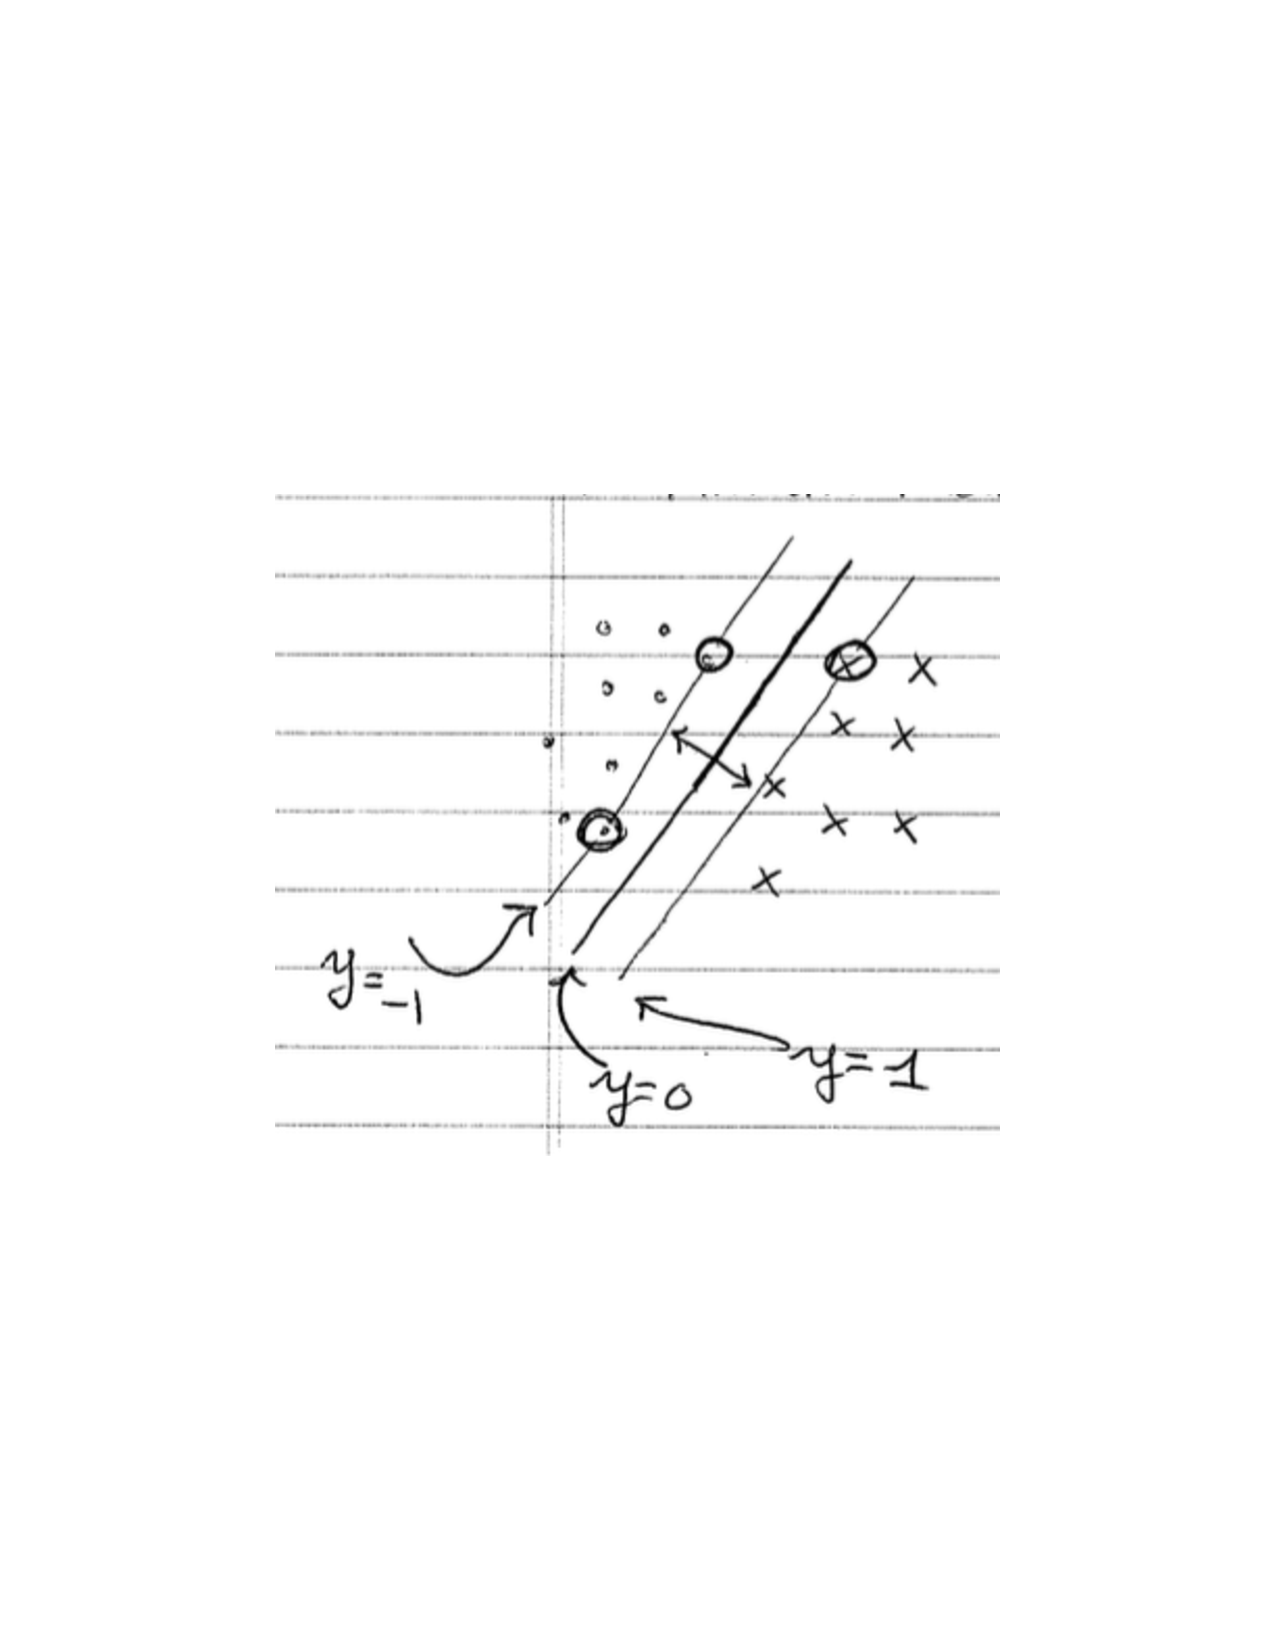
\includegraphics[width=3in, trim=5cm 8cm 5cm 8cm, clip=true]{svm_pic.pdf}\end{center}

\item We cannot directly compute $\phi(\x)$ for all mappings, we want to use a kernel trick.  So, we have to write up a dual representation of the problem in terms of $K$ matrices
\item We will start with the case where the $\phi(x)$ are linearly separable in the kernel space
\item Note: the SVM finds a linear decision boundary in the feature space.  But since we can do non-linear transformations to get to the feature space, the descision boundary can be non-linear in the feature space. 

\end{itemize}



\end{document} 